\section{Marco Teórico}
\subsection{Visión por computadora y su uso en la acuicultura}
La visión por computadora, también llamada visión artificial, es una disciplina dentro del aprendizaje de máquina y la informática que se centra en desarrollar algoritmos y sistemas capaces de interpretar y analizar imágenes y videos. Esto se logra mediante técnicas de procesamiento digital, modelado matemático, análisis de patrones y métodos estadísticos que permiten identificar objetos, segmentar escenas y comprender el contenido visual. Tiene aplicaciones prácticas en áreas como la robótica, la seguridad o la conducción autónoma.

La acuicultura constituye cerca de dos tercios de la producción de productos marinos en el mundo \cite{FAO2018} y la piscicultura forma parte importante de la actividad de acuicultura del país \cite{chile2017levantamiento}. Es entonces de vital importancia monitorear la integridad y salud de los peces por medio de revisiones regulares para asegurar una alimentación adecuada y la detección temprana de enfermedades. Lamentablemente, las mediciones manuales dependen de las condiciones meteorológicas, exigen mucho tiempo y trabajo y, sobre todo, son invasivas y estresantes para los peces \cite{Tonachella2022}.

Como solución alternativa se han propuesto métodos de estimación estadística para la talla de peces mediante sensores, radares y cámaras \cite{Tonachella2022} (Fig. \ref{fig:workflow_tonachella}), y el uso de modelos de aprendizaje automático en detección de enfermedades \cite{Ahmed2022}. Estas soluciones prometen ser más escalables, menos costosas e intervenir menos en el ciclo de vida de los animales.

\begin{figure}[htbp]
\begin{center}
    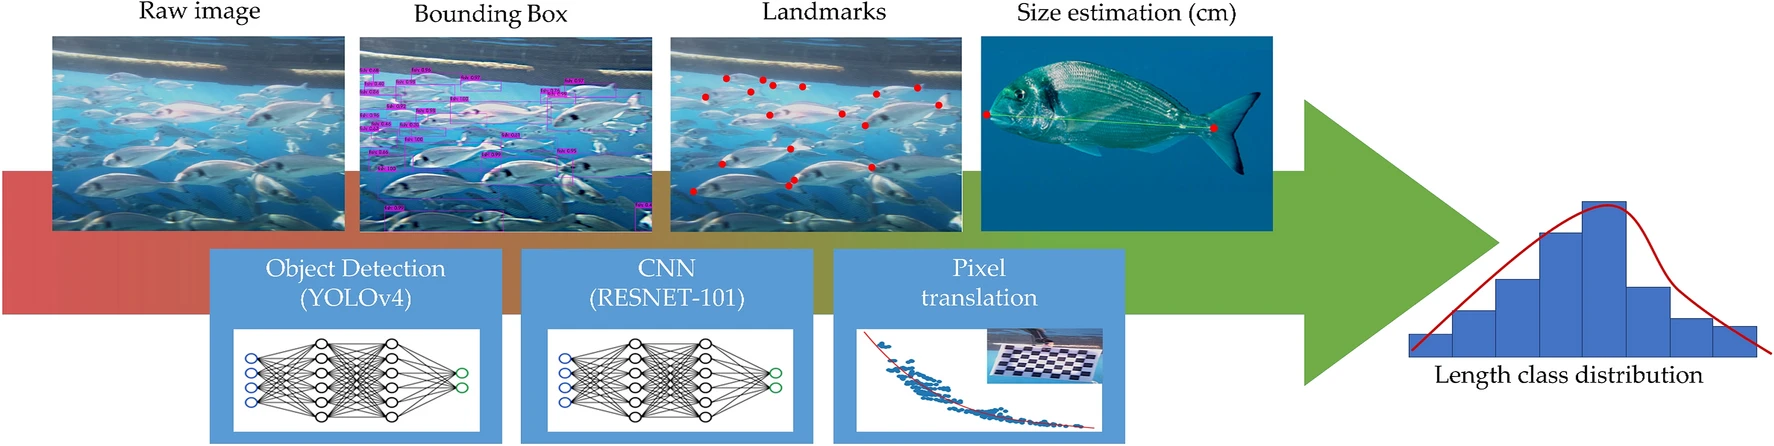
\includegraphics[width=0.9\textwidth]{figures/workflow_tonachella.png}
    \caption[Flujo de trabajo propuesto por Tonachella para estimación de la talla en peces]{Proceso general del método propuesto por Tonachella \cite{Tonachella2022}: reconocimiento automático por visión artificial y estimación de la talla en peces.}
    \label{fig:workflow_tonachella}
\end{center}
\end{figure}

WildSense por su parte implementa una novedosa técnica basada en el emparejamiento de mapas de profundidad obtenidos con cámaras estéreo y modelos tridimensionales generados en Blender, para la estimación de volumen y masa en peces.